\chapter{Implementierung der Parallelisierung}
\label{ch:Implementierung_Parallelisierung_Npp}
\chaptermark{Implementierung}

In diesem Kapitel wird zunächst die n++-Bibliothek und der bestehende Code vorgestellt, als auch auf den verwendeten Datensatz eingegangen. Anschließend werden die konzeptionellen Voraussetzungen erläutert und daraufhin wird die Implementierung detailliert vorgestellt. Dabei wird auch die Struktur der neuen Implementierung mit der der Vorarbeit verglichen.

\section{Erläuterung des n++-Simulatorkerns}
\label{sec:Erlauterung_Npp}
\sectionmark{Erläuterung n++}
N++ ist ein Simulator für neuronale Netze, der als Forschungsprojekt an der Universität Karlsruhe entwickelt wurde. Die Software ermöglicht die Simulation mehrerer neuronaler Netze und strebt danach, dem Anwender eine einfache Erweiterung der Grundfunktionen sowie eine benutzerfreundliche Schnittstelle für Anwendungsprogramme bereitzustellen \citep{Riedmiller_RPROP}.

Die Bibliothek n++ ist in C++ verfasst. Da sie seit über 20 Jahren besteht, verwendet sie größtenteils keine modernen C++-Features, unter anderem auch um die Kompatibilität mit C beizubehalten, da der Kern des Simulators auf dieser älteren Sprachversion aufbaut. Oft werden im Quellcode Funktionen der Standardbibliothek von C denen von C++ vorgezogen.

n++ ermöglicht es dem Benutzer, die Topologie des neuronalen Netzes zu spezifizieren und es an die spezifischen Anforderungen anzupassen. Hierbei können Parameter wie die Anzahl der Schichten, die Größe der Schichten sowie die Dimensionen der Ein- und Ausgabeschichten festgelegt werden \citep{dokumentation_npp}. Nach der Konfiguration des Netzes können Eingabemuster durch Vorwärtspropagation propagiert werden. Die resultierenden Ausgaben können abgerufen werden, und optional kann durch eine Rückführung des Fehlervektors ein Lernprozess des Netzes durchgeführt werden, wobei die Gewichte automatisch angepasst werden. Generierte Netze können in Dateien gespeichert werden, um sie zu einem späteren Zeitpunkt wiederzuverwenden, insbesonders für reproduzierbare Experimente.

In Codeausschnitt \ref{fig:npp_examplenet_code}, welcher eine vereinfachte Form des Beispielnetzes aus der n++-Dokumentation darstellt \citep{dokumentation_npp}, wird ein Beispielnetz mit drei Schichten erstellt. Die Eingabeschicht hat dabei zwei Parameter, die Ausgabeschicht drei, und die versteckte Schicht hat vier Parameter. Es ist ersichtlich, dass die n++-Bibliothek das einfache Austauschen von Updatefunktionen unterstützt. In den Zeilen 16 und 17 wird die Updatefunktion dynamisch auf Backpropagation gesetzt, was ohne großen Aufwand möglich ist.

\begin{figure}[H]
\begin{minted}
[
frame=lines,
framesep=2mm,
baselinestretch=1.2,
fontsize=\footnotesize,
linenos
]{c++}
#include "n++.h"

#define INPUTS 2
#define OUTPUTS 3
#define LAYERS 3

int main() {
    Net net;
    // Schichten des Netzes erstellen und miteinander verbinden
    int layerNodes[LAYERS] = {INPUTS, 4, OUTPUTS};
    net.create_layers(LAYERS, layerNodes);
    net.connect_layers();
    // Gewichte mit Zufallszahlen zwischen 0 und 0,5 initialisieren
    net.init_weights(0, 0.5);
    // Updatefunktion auf Rückwärtspropagation setzen
    float uparams[5] = {0.1, 0.9, 0, 0, 0};
    net.set_update_f(BP, uparams);
}
\end{minted}
\label{fig:npp_examplenet_code}
\caption{Vereinfachte Form des Beispielnetzes aus der n++-Dokumentation welche ein Netz mit 3 Schichten erstellt}
\end{figure}

\section{Bestehender Code}
\label{sec:Bestehender_Code_Brening}
\sectionmark{Bestehender Code}

Als bestehender Code wird ein Experiment aus der Bachelorarbeit von Artur Brening \citep{thesis_Artur_Brening} betrachtet. In dieser Bachelorarbeit wurde der Gradientenabstieg zum Trainieren neuronaler Netze implementiert. Dabei wurden viele Experimente mit verschiedenen Datensätzen und Lernmethoden zum Vergleich implementiert. Eines dieser Experimente wird als Grundlage für diese Bachelorarbeit übernommen.

Ausgewählt wurde das Experiment \enquote{MAGIC\_BP}, welches Rückwärtspropagierung nutzt. In dem Experiment wird der Magic Datensatz verwendet, auf welchen im Abschnitt \ref{sec:Datensatz} eingegangen wird. Es wird unter Einbindung der n++-Bibliothek ein neuronales Netz erstellt und zunächst ein festgelegter Teil des Datensatzes als Trainingsdatensatz genommen. Jede dieser Trainingsdaten wird zunächst vorwärts durch das neuronale Netz propagiert. Anschließend findet eine Fehlerbestimmung der resultierenden Ausgabe des Netzes statt, und der Fehlervektor rückwärtspropagiert.
Nachdem alle Datensätze aus dem Trainingsdatensatz vor- und rückwärtspropagiert wurden, definiert das Programm den verbleibende Teil des Datensatzes als Testdatensatz. Genau wie die Trainingsdatensätze wird jeder Datensatz zuerst vor- und dann rückwärts propagiert. Nach jedem Datensatz wird hier jedoch geprüft, ob die Klassifizierung des Netzes korrekt ist, um einen Überblick über den Anteil korrekt klassifizierter Datensätze zu schaffen.
Dieser Prozess wird für 10000 Epochen, also 10000 mal, über den gesamten Datensatz ausgeführt um das Netz lernen zu lassen.

Der beschriebene Ablauf läuft sequenziell für 10 verschiedene Netze mit jeweils verschiedenen Startseed ab, um das Verhalten mit verschiedenen Zufallszahlen zu überprüfen. Nachdem alle 10 Netze trainiert und getestet wurden, werden die Testergebnisse analysiert und in eine Datei geschrieben, um sie weiter verwerten zu können.

\begin{figure}[H]
\centering
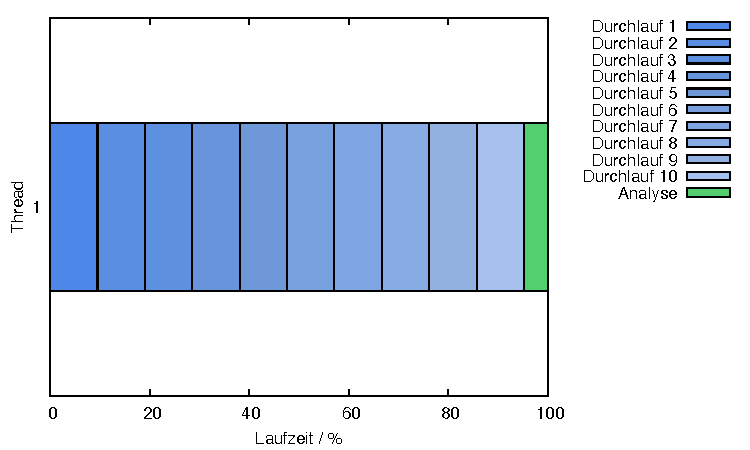
\includegraphics[width=0.8\textwidth]{../results/plots/timeline/timeline_plot_1thread.pdf}
\caption{Schematischer Ablauf des bestehenden Programms. In jedem Durchlauf wird ein neuronales Netz mit 10000 Epochen trainiert und anschließend getestet. In der Analyse werden die Ergebnisse aller Netze zusammengetragen und in eine Datei geschrieben.}
\label{fig:timeline_existing_code}
\end{figure}

Wie in Abbildung \ref{fig:timeline_existing_code} ersichtlich laufen alle Netze, auf der Grafik in blau dargestellt, auf einem Thread. Anschließend wird die Analyse, in grün dargestellt, ausgeführt. In dieser Arbeit werden die Trainings- und Testdurchläufe parallelisiert, was bedeutet, dass potenziell 10 Netze gleichzeitig trainiert und getestet werden können. Dies könnte möglicherweise zu großen Leistungsverbesserungen führen, da das Training und Testen der Netze den Großteil der Laufzeit einnimmt, und die Analyse nur wenige Sekunden in Anspruch nimmt. 

\section{Datensatz}
\label{sec:Datensatz}
\sectionmark{Datensatz}

Der verwendete Datensatz MAGIC Gamma Telescope aus dem UCI Machine Learning Repository ist eine bedeutende Ressource für die Forschung im Bereich der Gamma-Teleskopie. Er enthält eine Vielzahl von Beobachtungen, die von Gammastrahlen-Teleskopen gemacht wurden. Jede Beobachtung wird durch eine Reihe von Merkmalen beschrieben, die aus den gemessenen Eigenschaften der Gammastrahlen stammen. Das Hauptziel bei der Verwendung dieses Datensatzes ist die Klassifizierung von Beobachtungen in verschiedene Kategorien oder Klassen. Durch die Anwendung von Klassifizierungsalgorithmen können Muster und Zusammenhänge in den Daten identifiziert werden, was wiederum dazu beitragen kann, das Verständnis der Gammastrahlenphänomene im Universum zu vertiefen \citep{misc_magic_gamma_telescope_159}. Das UCI Machine Learning Repository ist eine bekannte Datenbank, die eine Vielzahl von Datensätzen für die Forschung und Entwicklung im Bereich des maschinellen Lernens bereitstellt. Die Daten sind kostenfrei verfügbar und können für verschiedene Zwecke verwendet werden. Der Datensatz enthält insgesamt 19020 Beobachtungen \citep{misc_magic_gamma_telescope_159}.

\section{Voraussetzungen}
\label{sec:Voraussetzungen_Parallelisierung}
\sectionmark{Voraussetzungen}
Für eine erfolgreiche Parallelisierung des Anwendercodes ist eine umfassende Analyse und Modifikation desselben unerlässlich. Dieser Abschnitt diskutiert die grundlegenden Voraussetzungen, die vor der Implementierung von Parallelisierungsstrategien berücksichtigt werden müssen. In erster Linie erfordert die Parallelisierung die Identifizierung und Beseitigung von Abhängigkeiten innerhalb des Algorithmus sowie die Anpassung der Implementierung, um die Effizienz und Skalierbarkeit auf mehreren Prozessoren oder Rechenkernen zu gewährleisten \citep{wilkinson2006parallel}.

\subsection{Entfernung von geteilten Speicherzugriffen}
\label{sec:Entfernung_geteilte_Speicherzugriffe}
Geteilte Speicherzugriffe, auch Shared Memory genannt, häufig realisiert durch globale Variablen im Quellcode, ermöglichen es verschiedenen Teilen eines Programms, auf dieselben Daten zuzugreifen. Diese Abhängigkeit ermöglicht es dem Programmierer, komplexe Algorithmen simpel zu implementieren. Während dies in einer sequenziellen Umgebung einigermaßen gut funktionieren kann, können Probleme auftreten, wenn versucht wird, solche Konstrukte in einem parallelen Kontext zu verwenden.

Bei der Parallelisierung eines Programms ist es entscheidend, dass verschiedene Threads oder Prozesse unabhängig voneinander arbeiten können, um eine effiziente und sichere Ausführung zu gewährleisten. Globale Variablen führen jedoch schnell zu potenziellen Konflikten, da mehrere Threads gleichzeitig auf denselben Speicherbereich zugreifen können. Dies kann zu Wettlaufsituationen, inkonsistenten Zuständen und anderen unerwarteten Verhaltensweisen führen, die die Zuverlässigkeit und Korrektheit des Programms beeinträchtigen \citep{Czech_2017_Shared_Memory}.

Um dieses Problem zu lösen, ist es notwendig, die Abhängigkeit von geteilten Speicherzugriffen so weit wie möglich zu reduzieren. Dies erfolgt durch die Umstrukturierung des Quellcodes, um den Einsatz globaler Variablen zu minimieren oder ganz zu eliminieren. Statt globaler Variablen können lokale Variablen verwendet werden, die nur innerhalb bestimmter Funktionsbereiche gültig sind und somit den Zugriff auf den Speicher einschränken. Diese Vorgehensweise kann zusätzlich Vorteile in Bezug auf Speicherlecks und Speicherbedarf mit sich bringen, da die Variablen nur für die Zeit ihrer Verwendung im Hauptspeicher vorhanden sind. Darüber hinaus können Datenstrukturen wie Klassen oder Strukturen verwendet werden, um Daten zu kapseln und den Zugriff über klar definierte Schnittstellen zu ermöglichen \citep{Czech_2017_Shared_Memory}.

Bei der Entfernung von geteilten Speicherzugriffen ist es wichtig, auch geeignete Synchronisationsmechanismen einzuführen, um kritische Abschnitte des Codes zu schützen. Dies kann die Verwendung von Mutexen, Semaphoren oder anderen Mechanismen umfassen, um sicherzustellen, dass nur ein Thread gleichzeitig auf bestimmte Ressourcen zugreifen kann, und so potenzielle Wettlaufbedingungen zu vermeiden. Die Verwendung von Mutexen sollte jedoch nicht ohne Vorbehalt in Erwägung gezogen werden, da sie weitere Abhängigkeiten schafft, welche die Leistungsgewinne durch mehrere Threads wieder negieren könnten. Ist dies der Fall, sollte über eine größere Umstrukturierung der Architektur nachgedacht werden, um das Programm mit Parallelisierung kompatibel zu machen \citep{Czech_2017_Shared_Memory}.

\subsection{Verlagerung der zu parallelisierenden Routine}
\label{sec:Verlagerung_parallelisierende_Routine}
Um eine effektive Parallelisierung zu erreichen, ist es von entscheidender Bedeutung, den spezifischen Teil des Codes zu identifizieren, der für die parallele Ausführung geeignet ist. Dieser Prozess erfordert eine sorgfältige Analyse des Quellcodes, um Bereiche zu lokalisieren, die unabhängig voneinander ausgeführt werden können und keine oder nur minimale Abhängigkeiten zu anderen Teilen des Programms aufweisen. Solche Bereiche können typischerweise Schleifen oder Abschnitte sein, die große Mengen von Daten verarbeiten, ohne auf Zwischenergebnisse anderer Bereiche angewiesen zu sein. Gegebenenfalls kann es auch sinnvoll sein, mit einem Profiler die Laufzeit des Programms zu analysieren, um zutreffende Teile zu identifizieren \citep{wilkinson2006parallel}.

Nachdem der geeignete Bereich identifiziert wurde, ist es notwendig, ihn aus dem Hauptcode auszulagern und in eine separate Routine oder Funktion zu überführen. Diese ausgelagerte Routine sollte autonom arbeiten können, ohne auf globale Variablen oder gemeinsam genutzte Ressourcen außerhalb ihres Bereichs zuzugreifen. Durch diese Isolierung können potenzielle Konflikte vermieden und die Parallelisierung erleichtert werden \citep{wilkinson2006parallel}.

Es ist essenziell sicherzustellen, dass die ausgelagerte Routine keine Abhängigkeiten zu anderen Teilen des Codes hat, um eine effiziente Parallelisierung zu ermöglichen. Hierbei müssen gegebenenfalls erforderliche Parameter übergeben und Rückgabewerte behandelt werden, um eine reibungslose Interaktion mit dem Rest des Programms zu gewährleisten \citep{wilkinson2006parallel}.

Die Verlagerung der zu parallelisierenden Routine ist mitunter der wichtigste Schritt bei der Implementierung von Parallelisierungsstrategien und bildet die Grundlage für eine effiziente und robuste parallele Ausführung des Programms. Durch die Identifizierung und Isolierung geeigneter Bereiche können potenzielle Engpässe reduziert und die Leistung des Programms optimiert werden.

Unter Umständen ist es nicht ohne Weiteres möglich, einfach einen bestimmten Teil des bestehenden Quellcodes auszulagern und diesen zu parallelisieren. Ist dies der Fall, so muss der Quellcode allgemein konzeptionell umstrukturiert werden. In der Praxis ist dies einer der größten Faktoren, die zur Komplexität von Parallelisierung beitragen.

\section{Vorstellung der Implementierung}
\label{sec:Vorstellung_Implementierung}

In dieser Sektion wird die Implementierung vorgestellt, wobei einige Aspekte im Anschluss genauer beleuchtet werden. Einige Code-Segmente werden im Vergleich mit der vorherigen Implementierung dargestellt, um die Veränderungen zu veranschaulichen.

Die Herangehensweise der Implementierung war es, zunächst eigenständige Code-Segmente in Funktionen auszulagern, um die Verantwortung einzelner Funktionen klar zu definieren, und große Funktionen mit viel Code herunterzubrechen. Dies ermöglicht es, einfacher zu identifizieren, welche Segmente sich möglicherweise für eine parallele Durchführung eignen. Für die Verlagerung von Code in eigene Funktionen ist es erforderlich, Übergabewerte und Rückgabewerte dieser Funktionen zu definieren, um weiterhin auf die Daten zugreifen zu können. Dabei wurde bereits darauf geachtet, alle neuen Funktionen ohne Seiteneffekte zu implementieren, was bedeutet, dass sie keine externen Zustände verändern und für gegebene Übergabewerte immer die gleichen Rückgabewerte erzeugen. Dies ist für die Strukturierung des Codes für die Parallelisierung von großem Vorteil.

Bei der Analyse stellte sich recht schnell heraus, dass sich der Abschnitt, in welchem ein neuronales Netz zunächst trainiert und dann getestet wird, am besten für die Parallelisierung eignet. Dieser Abschnitt wurde in eine Funktion namens \glqq\text{runSeed}\grqq ausgelagert. Die Funktion bekommt den auszuführenden Seed und den gesamten Datensatz, der bei Programmstart einmalig eingelesen, in Zeilen aufgeteilt und deserialisiert wird, übergeben. Dies unterscheidet sich von der bestehenden Implementierung, in welcher der Datensatz bei jedem Durchlauf mehrfach zerteilt und eingelesen wird, worauf in der nächsten Sektion \ref{sec:Verwendung_threadsichere_Funktionen} genau eingegangen wird. Dies hat auch Leistungsimplikationen, da der überarbeitete Ansatz nicht nur threadsicher, sondern auch performanter ist.

\subsection{Verwendung von threadsicheren Funktionen}
\label{sec:Verwendung_threadsichere_Funktionen}

Besonders zur Manipulation von Zeichenketten macht sowohl die n++-Bibliothek als auch der Code des Experimentes von Herrn Brening viel von klassischen Funktionen aus der C-Standardbibliothek Gebrauch. Beispielsweise wird wie in Abbildung \ref{fig:strtok_usage_before} zu sehen in der n++-Bibliothek die Funktion strtok verwendet, welche eine Zeichenkette tokenisieren kann, um ein neuronales Netz aus einer Datei zu laden und zu deserialisieren.

\begin{figure}[H]
\begin{minted}
    [
    frame=lines,
    framesep=2mm,
    baselinestretch=1.2,
    fontsize=\footnotesize,
    linenos,
    firstnumber=611
    ]
    {c++}
int Net::load_net( char filename[] ) {
    ...
    else if (strncmp(line,"topology",7)==0){
        value=strtok(line, " \t\n");  /* skip first token (== topology)*/
        for(i=0,value=strtok( NULL," \t" );(value!=NULL)&&(i<MAX_LAYERS);
        value=strtok( NULL," \t\n" ),i++){
    ...
\end{minted}
\label{fig:strtok_usage_before}
\caption{Ausschnitt aus dem bestehenden Code der N++ Bibliothek, in welchem viel Gebrauch von der strtok-Funktion gemacht wird.}
\end{figure}

Werden mehrere Netze gleichzeitig geladen, kann die Verwendung von strtok in diesem Kontext jedoch zu Problemen und Konflikten führen, da die strtok-Funktion intern den Zustand der Zeichenkettenzerteilung speichert, um bei folgenden Aufrufen den nächsten Teil der Zeichenkette zurückzugeben. Wenn die Funktion also an mehreren Stellen gleichzeitig aufgerufen wird, entstehen inkonsistente Ergebnisse. Für diese Fälle existiert in der Standardbibliothek zum Beispiel die Funktion strtok\_r, welche ähnlich wie strtok funktioniert, den internen Zustand jedoch in einem Pointer speichert, und es somit ermöglicht in jedem Thread einen separaten Pointer zu benutzen \citep{Posix_Specification}. Der Code musste in diesem Fall leicht umstrukturiert werden, danach ist er aber threadsicher. Das Ergebnis ist in Abbildung \ref{fig:strtok_r_usage_after} ersichtlich.

\begin{figure}[H]
\begin{minted}
    [
    frame=lines,
    framesep=2mm,
    baselinestretch=1.2,
    fontsize=\footnotesize,
    linenos,
    firstnumber=611
    ]
    {c++}
int Net::load_net( char filename[] ) {
    ...
    char *saveptr; // Speichert den Zustand der Tokenisierung der Zeichenkette
    ...
    else if (strncmp(line, "topology", 7) == 0) {
        strtok_r(line, " \t\n", &saveptr); /* skip first token (== topology)*/
        for (i = 0, value = strtok_r(nullptr, " \t", &saveptr);
             (value != nullptr) && (i < MAX_LAYERS);
             value = strtok_r(nullptr, " \t\n", &saveptr), i++) {
    ...
\end{minted}
\label{fig:strtok_r_usage_after}
\caption{Ausschnitt aus dem überarbeiteten Code der N++ Bibliothek, in welchem die strtok-Funktion durch die strtok\_r-Funktion ersetzt wurde.}
\end{figure}

Diese Verwendung von strtok tritt sehr häufig in dem n++-Quellcode auf. Auch in dem Code von Herrn Brening wird strtok verwendet, um den Datensatz einzulesen, und die relevanten Parameter zu extrahieren. Jeder dieser Funktionsaufrufe wurde durch threadsichere Alternativen wie strtok\_r ersetzt.
Weitere häufige verwendete Beispiele für thread-unsichere Funktionen der Standardbibliothek, sind asctime, ctime und localtime, aber auch die Zufallsgeneratorfunktionen wie rand und srand.
Wichtig zu erwähnen ist jedoch, dass je nach Anwendungsfall die threadsicheren Funktionen wie strtok\_r nicht verfügbar sein könnten, zum Beispiel, wenn man die Portabilität für POSIX-Systeme vor 2001 gewährleisten möchte \citep{Posix_Specification}.

Um das Nachvollziehen des Programmablaufs zu vereinfachen, verfügte die bestehende Implementierung über viele Konsolenausgaben welche mit cout und dem <<-Operator von C++ realisiert worden sind. Diese Konsolenausgaben sind nicht threadsicher, da die Konkatenation von Zeichenketten bei gleichzeitigen Aufrufen die Daten verschiedener Threads sofort ausgegeben werden, bevor sie konkateniert wurden. Als Lösung wurde in der parallelisierten Implementierung die printf Funktion genutzt, welche die Zeichenkette zuerst formattiert und konkateniert, bevor sie in der Konsole ausgegeben wird. Diese Änderung führt jedoch auch zu geringen Leistungsunterschieden, da die Funktionsweise beider Methoden nicht vergleichbar ist.

\subsection{Entfernung globaler Variablen}
\label{sec:Entfernung_globaler_Variablen}

In der bestehenden Implementierung von Herrn Brening, von der ein Teil in Abbildung \ref{fig:global_variable_usage_before} zu sehen ist, werden die meisten Variablen global, also außerhalb von Funktionen und Klassen, definiert. Die Verwendung von globalen Variablen ermöglicht eine subjektiv empfundene höhere Lesbarkeit und Verständlichkeit des Quellcodes, da alle verwendeten Variablen zu Beginn der Datei definiert sind und somit an einer Stelle eingesehen werden können. Des Weiteren ermöglichen globale Variablen eine Reduzierung von Parameterübergaben in Funktionen, da auf sie von allen Funktionen direkt zugegriffen werden kann.

\begin{figure}[H]
\begin{minted}
[
frame=lines,
framesep=2mm,
baselinestretch=1.2,
fontsize=\footnotesize,
linenos,
firstnumber=24,
]
{c++}
Net* net;
string* trainingData;
string* testingData;
int dataSetCount;
int seed;

int topology[LAYERS];
float uparams[10];
FTYPE *in_vec, *out_vec, *tar_vec;
\end{minted}
\caption{Teil der globalen Variablendefinition in der bestehenden Implementierung von Herr Brening}
\label{fig:global_variable_usage_before}
\end{figure}

Die globalen Variablen werden für die Datensätze, das neuronale Netz und die Propagierung von Daten verwendet. Im Kontext der Parallelisierung entstehen durch diese Verwendung von globalen Variablen jedoch Konflikte, welche ein Beibehalten dieser Struktur unmöglich machen. So entstehen beispielsweise geteilte Speicherzugriffe wie bereits in Sektion \ref{sec:Entfernung_geteilte_Speicherzugriffe} angesprochen, da nun mehrere Netze zeitgleich laufen sollen. So müsste es beispielsweise entweder eine Variable für jedes Netz geben, oder man schützt die Zugriffe beispielsweise mit einem Mutex, was die Parallelisierung jedoch unwirksam machen würde. Deshalb wurde sich entschieden, die globalen Variablen zu entfernen, und erst an der Stelle zu definieren, wo sie verwendet werden. Das neuronale Netz und die Vektoren werden in Abbildung \ref{fig:local_variable_usage_after} beispielsweise erst innerhalb eines Threads definiert, sodass jeder Thread und jeder Ablauf über separate Netze verfügt, was die Konflikte beseitigt.

\begin{figure}[H]
    \begin{minted}
    [
    frame=lines,
    framesep=2mm,
    baselinestretch=1.2,
    fontsize=\footnotesize,
    linenos,
    firstnumber=242,
    ]
    {c++}
static void runSeed(const int seed, const vector<DatasetRow> &trainingset,
 const vector<DatasetRow> &testingset) {
    ...
    const auto net = new Net();
    ...
    const auto inVec = new float[net->topo_data.in_count];
    const auto outVec = new float[net->topo_data.out_count];
    const auto tarVec = new float[net->topo_data.out_count];
\end{minted}
\caption{Verlagerung der globalen Variablen zu lokalen Variablen in der parallelen Implementierung.}
\label{fig:local_variable_usage_after}
\end{figure}

Die globalen Variablen, welche die Ergebnisse der Experimente speichert, mussten nicht entfernt werden, da bereits 10, also eine für jeden Seed bestehen. Der Code wurde vereinfacht, da dem Array stattdessen eine weitere Dimension hinzugefügt wurde, die spezifiziert, von welchem seed die Ergebnisse stammen. So wurde der Code lesbarer, und es gibt weiterhin getrennte Speichersegmente für verschiedene Threads.

\subsection{Verwendung eines Threadpools}
\label{sec:Verwendung_Thread_Pool}

Ein Threadpool ist ein Entwurfsmuster, das häufig in der parallelen Programmierung verwendet wird, um die Verteilung von Aufgaben auf eine gewisse Anzahl an Threads zu vereinfachen. Ein Threadpool besteht aus einer festgelegten Anzahl von vorab initialisierten Threads, die darauf warten, Aufgaben auszuführen. Sobald eine Aufgabe an den Threadpool übergeben wird, wird sie von einem verfügbaren Thread ausgeführt, während andere Threads weiterhin bereitstehen, um zusätzliche Aufgaben zu übernehmen \citep{ThreadPool_Tutorial_Cpp}. Dieses Konzept trägt dazu bei, die Kosten für die Erstellung und Zerstörung von Threads zu minimieren und die Systemressourcen effizient zu nutzen. Die Funktionsweise eines Threadpools kann wie folgt beschrieben werden:
\begin{enumerate}
    \item Initialisierung: Ein genaue Anzahl von Threads wird beim Start des Programms erstellt und in Bereitschaft gehalten.
    \item Aufgabenzuweisung: Aufgaben werden einer Warteschlange hinzugefügt, die vom Threadpool verwaltet wird.
    \item Aufgabenausführung: Verfügbare Threads nehmen Aufgaben aus der Warteschlange und führen sie aus.
    \item Rückführung: Nach der Ausführung einer Aufgabe kehrt der Thread in den Pool zurück und wird für neue Aufgaben bereitgestellt.
    \item Terminierung: Stehen keine weiteren Aufgaben an und wird eine Terminierungsfunktion aufgerufen, fährt der Threadpool geordnet herunter, indem laufende Aufgaben abgeschlossen und anschließend die Threads beendet werden. Die Terminierung kann blockierend oder nicht-blockierend implementiert sein, abhängig von den Anforderungen der Anwendung.
\end{enumerate}

Ein Threadpool ermöglicht eine kontrollierte Anzahl von gleichzeitig ausgeführten Threads, wodurch Probleme wie übermäßige Thread-Erstellung und Ressourcenkonflikte vermieden werden. Durch die Begrenzung der Anzahl aktiver Threads können die Systemressourcen effizienter genutzt und die Stabilität des Systems gewährleistet werden. Stehen beispielsweise nur 2 Kerne zur Verfügung, ist es in vielen Fällen effizienter, die Aufgaben von 2 Threads abarbeiten zu lassen, anstatt 50 Threads gleichzeitig zu starten. Zudem wird die Verwaltung von Threads zentralisiert und vereinfacht, da der Threadpool die Lebenszyklen der Threads und die Aufgabenzuweisung übernimmt.

Da die C++-Standardbibliothek nicht über einen ThreadPool verfügt, wurde eine Implementierung aus dem Internet verwendet \citep{ThreadPool_Tutorial_Cpp}. Der verwendete ThreadPool ist simpel aufgebaut, und in einer einzigen C++-Header-Datei implementiert. Abbildung \ref{fig:threadpool_example_usage} zeigt ein Beispielprogramm, welches den Threadpool verwendet.

\begin{figure}[H]
\begin{minted}
        [
        frame=lines,
        framesep=2mm,
        baselinestretch=1.2,
        fontsize=\footnotesize,
        linenos,
        ]
        {c++}
#include "threadpool/threadpool.h"

int main() {
    // Threadpool mit 2 Threads erstellen
    ThreadPool *threadpool = new ThreadPool(2);
    // 50 Beispielaufgaben erstellen und der Warteschlange hinzufügen
    for (int i = 1; i <= 50; i++) {
        threadpool->enqueue([i] { // Abhängigkeiten müssen spezifiziert werden
            printf("Aufgabe %d\n", i);
        });
    }
    // Aufruf des Destruktors terminiert Threads nach Abschluss aller Aufgaben
    delete threadpool;
    return 0;
}
\end{minted}
\caption{Beispielhafter C++-Code zur Verwendung eines Threadpools: Ein Threadpool mit zwei Threads wird erstellt, 50 Aufgaben werden der Warteschlange hinzugefügt und anschließend wird der Threadpool blockierend terminiert.}
\label{fig:threadpool_example_usage}
\end{figure}
    
In dieser Arbeit wird der Threadpool verwendet, um das Trainieren und Testen der einzelnen neuronalen Netze auf mehrere Kerne zu verteilen. Es handelt sich folglich immer um 10 Aufgaben, welche der Warteschlange des Threadpools hinzugefügt werden. Die genaue Verteilung der Aufgaben auf die verfügbaren Threads wird im nächsten Kapitel erläutert.